\chapter{Implementierung}
\label{implementierung}
\renewcommand{\arraystretch}{1.2}
\newcolumntype{a}{>{\centering\arraybackslash}m{(\linewidth)/2}|}

In diesem Kapitel wird die Implementierung beschrieben. Zunächst werden die Komponenten und Klassen der Anwendung vorgestellt. Die gezeichneten Mockups unterscheiden sich nur minimal von der tatsächlichen Anwendung. Im Großen und Ganzen ist das Design aber gleich geblieben, was bei Betrachtung von \autoref{fig:app} auffällt.

\begin{figure}[h!]
	\centering
	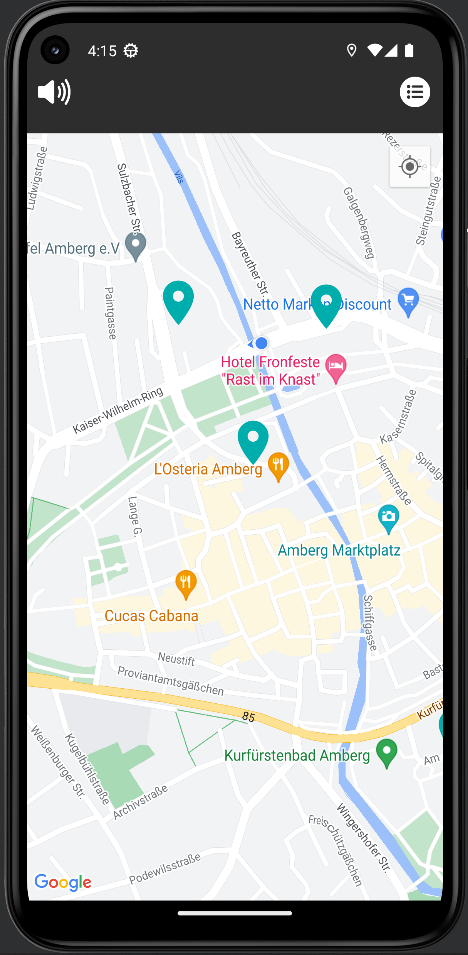
\includegraphics[width=0.3\linewidth]{app.png}
	\caption[Die Startseite der fertigen Anwendung, auf welcher nun die Parkmöglichkeiten zu sehen und durch Klick auf einen der türkisblauen Marker nähere Informationen zu finden sind. Oben rechts kann auch eine Liste der Parkmöglichkeiten aufgerufen werden. In der linken oberen Ecke kann der Ton an- und ausgeschaltet werden.]
	{Die Startseite der fertigen Anwendung, auf welcher nun die Parkmöglichkeiten zu sehen und durch Klick auf einen der türkisblauen Marker nähere Informationen zu finden sind. Oben rechts kann auch eine Liste der Parkmöglichkeiten aufgerufen werden. In der linken oberen Ecke kann der Ton an- und ausgeschaltet werden. (Quelle: Screenshot der erstellten Anwendung.)}
	\label{fig:app}
\end{figure}
\newpage

Die genutzten Farben werden generiert. Grundlage ist die zuvor ausgewählte dunkelgraue Hintergrundfarbe. So wird sichergestellt, dass die Farben auch wirklich zusammenpassen \cite{colors}. Eine Bibliothek für die Icons ist standardmäßig bei Expo-Projekten integriert, dennoch müssen die Bezeichnungen zu den passenden Icons gefunden werden, was über die react-native-vector-icons-Directory gut geklappt hat \cite{icons}.
\section{Komponenten}
Die Komponenten bilden alle Funktionen der App, welche visuell auf der Benutzeroberfläche wahrgenommen werden. Neben der Anzeige der Elemente beinhalten sie aber dennoch auch Funktionalität, wie beispielsweise das Aufrufen von Methoden der Datenbank-Klasse ,DbConnectionService'. Alle Komponenten, mit Ausnahme der ,App', besitzen ein eigenes Interface. Dieses Interface beinhaltet alle Elemente, die als Properties in die Komponente hineingegeben werden und die jeweils dazugehörigen Typen. Properties können als Parameter einer Komponente verstanden werden. Dies können neben Strings, Zahlenwerten oder boolschen Werten auch Funktionen oder andere Objekte sein.
\subsection{Komponente ,App'}
Die ,App'-Komponente kann sozusagen mit der ,main()'-Funktion anderer Programmiersprachen verglichen werden. Alles, was in dieser Funktion seinen Platz findet, findet sich auch in der Anwendung selbst wieder. Alle notwendigen Komponenten, die die Anwendung benötigt, werden hier eingefügt. 

Zu Beginn werden hier die Tabellen der Datenbank erstellt, sofern diese noch nicht existieren. Diese Komponente verwaltet aber auch Daten. Die Informationen zu den Parkmöglichkeiten, die über die API abgerufen werden, werden beispielsweise auch hier verwaltet. Durch den Hook ,useEffect' wird sichergestellt, dass die Daten nach einer bestimmten Zeit erneut abgefragt werden. Der Code hierfür kommt aus dem Internet und ist in \autoref{lst:useEffectApiData} zu sehen.

\begin{lstlisting}[caption={In diesem ,useEffect'-Hook werden nach der Zeit, welche sich hinter der Variable ,MINUTES\_MS' verbirgt, die Daten der API abgerufen, was über die Funktion in Zeile 3 geschieht. (Quelle: \cite{useIntervalCode})},captionpos=b, language=Java, label=lst:useEffectApiData]
	useEffect(() => {
		const intervalCall = setInterval(() => {
			dbConnectionService.getData();
		}, MINUTES_MS);
		return () => {
			clearInterval(intervalCall);
		};
	}, []);
\end{lstlisting}

Desweiteren gehen auch die Daten des Eventhooks ,useGeofenceEvent', welcher in \autoref{geofenceEvent} erklärt wird, hier ein. Durch die Properties der anderen Komponenten werden die Daten dann an die richtigen Stellen gebracht. Wird ein Geofence betreten, so geschieht auch hier die Sprachausgabe. Der Button für das Ein- und Ausschalten des Tons befindet sich ebenfalls in der ,App'. Auch die Verwaltung des Tons liegt hier. Wird eine andere Ansicht geöffnet oder der Button zum Stummschalten der Sprachausgabe betätigt, so wird ein ,useEffect'-Hook getriggert, welcher die Sprachausgabe direkt beendet.

Neben verschiedenen ,set'- und ,get'-Funktionen, die für die Weitergabe von Daten zwischen Komponenten verantwortlich sind, befindet sich hier auch das Element, welches benötigt wird, um Toasts auszugeben. Alle Bestandteile in der ,View'-Komponente werden von ,<RootSiblingParent>' umrahmt, damit nachher an verschiedenen Stellen der Befehl aus \autoref{lst:toast} aufgerufen werden kann und somit in der Anwendung einen Toast anzeigt \cite{toastLibrary}.

\begin{lstlisting}[caption={Ein Beispiel des Aufrufs eines Toasts aus der Datei ,DbConnectionService.ts'. (Quelle: Eigene Implementierung)},captionpos=b, language=Java, label=lst:toast]
	Toast.show(errorMessages.noApiConnectionMessage, {
		duration: Toast.durations.LONG,
		position: Toast.positions.BOTTOM,
	});
\end{lstlisting}

\subsection{Komponente ,ParkingMap'}
Die wohl wichtigste Komponente der Anwendung ist die, welche die Karte beinhaltet. Diese findet sich hier. Zunächst wird beschrieben, welche Properties mitgeliefert werden. Hierzu ist es hilfreich, das zugehörige Interface ,IParkingMap' mit den Typen der Properties zu betrachten:
\begin{description}
	\item \textbf{handleParkingAreaId(id: number): void} \\ Hineingegeben wird eine Funktion ,handleParkingAreaId', welche nichts zurückgibt. Parameter ist hier ,id', was den Typ Nummer hat. Diese Funktion bringt die jeweilige ID der Parkmöglichkeit nach draußen in die ,App' und kann dort weiterverarbeitet werden.
	\item \textbf{handleParkingAreaDescription(parkingAreaDescription: boolean): void} \\ ,handleParkingAreaDescription' ist eine Funktion, welche nichts zurückgibt. Der Parameter dieser Funktion ist ein boolscher Wert namens ,parkingAreaDescription'. Diese Property hat in etwa denselben Nutzen, wie die eben beschriebene. Nur wird hier der ,App' mitgeteilt, ob die Beschreibung einer Parkmöglichkeit geöffnet werden soll oder nicht.
	\item \textbf{mapStyle: StyleProp<ViewStyle>} \\ Diese Property ist für das Design der ,ParkingMap' verantwortlich. Je nachdem, ob die Beschreibung der Parkmöglichkeit angezeigt wird oder nicht, ist die ,ParkingMap' größer oder kleiner.
\end{description}

Diese Komponete übernimmt die Anzeige der aktuellen Position des Nutzers und das Bilden der Geofences. Damit das funktioniert, wird die Bibliothek Location von expo benötigt \cite{expoLocation}. Zur Nutzung von Geofences und der Anzeige der aktuellen Position wird die Erlaubnis des Nutzers für das GPS benötigt. Ohne diese Zustimmung wird dem Nutzer eine Meldung angezeigt, dass weder das Geofencing, noch die Anzeige der aktuellen Position funktionieren. Damit das Geofencing funktionieren kann, muss mit Hilfe der Expo-Bibliothek Task-Manager der mit einem Namen definierte Task gefunden werden, der das Geofencing startet \cite{taskmanager}.

Um nun auch die Karte und die Marker an den Positionen der Parkmöglichkeiten anzeigen zu lassen, werden zusätzlich die Komponenten ,MapView' und ,Marker' der Bibliothek ,react-native-maps' benötigt. Je nach Gerät wird dann bei Android Google Maps und bei IOS Apple Maps verwendet. Um nun die Marker an den richtigen Stellen zu plazieren, wird die Liste aller Objekte der Parkmöglichkeiten mit der Funktion ,map()' durchgegangen und an jeder Stelle der Parkhäuser ein Marker gesetzt. Die Daten der Parkhäuser sind hier nicht aus der Datenbank, sondern aus dem Objekt-Array ,AllParkingAreas', welches in \autoref{AllParkingAreas} näher erklärt wird. Wird auf einen Marker geklickt, kommen die beiden Funktionen der Properties ins Spiel. Der Aufruf der Funktion ,handleParkingAreaId' mit der ID der angeklickten Parkmöglichkeit als Parameter lässt die ,App' wissen, welche Parkmöglichkeit angeklickt wurde. Wenn die Funktion ,handleParkingAreaDescription' mit dem Parameter ,true' aufgerufen wird, wird sichergestellt, dass sich dann immer die Beschreibung, welche in \autoref{fig:parkingAreaDescription} zu sehen ist, öffnet.

\begin{figure}[h!]
	\centering
	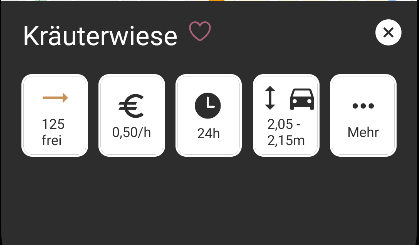
\includegraphics[width=0.45\linewidth]{parkingAreaDescription_component.png}
	\caption[Die Komponente ,ParkingAreaDescription', welche bei Klick auf einen Marker aufgerufen wird.]
	{Die Komponente ,ParkingAreaDescription', welche bei Klick auf einen Marker aufgerufen wird. (Quelle: Screenshot der erstellten Anwendung.)}
	\label{fig:parkingAreaDescription}
\end{figure}

\subsection{Komponente ,ParkingAreaDescription'}
\label{handleFunctions}
In dieser Komponente werden die relevantesten Daten einer Parkmöglichkeit in Kacheln angezeigt, wie in \autoref{fig:parkingAreaDescription} zu sehen ist. Auch für die Properties dieser Komponente gibt es ein Interface ,IParkingAreaDescription':
\begin{description}
	\item \textbf{dbConnectionService: DbConnectionService} \\ Dies ist eine Instanz des ,DbConnectionService', welche in der ,App' am Anfang erstellt wird. Diese Property ist für die Datenbankverbindung zuständig.
	\item \textbf{id: number} \\ Mit der Nummer ID kommt die ID der angeklickten Parkmöglichkeit in die Beschreibung. Nun kann mit Hilfe von ,dbConnectionService' in der Datenbank nach den passenden Daten gesucht werden.
	\item \textbf{geofenceEventData: IEventData[]} \\ Die Daten des Events ,useGeofenceEvent' werden jeweils in einem Objekt mit dem Interface ,IEventData' gespeichert. Jedes Objekt, was eine Parkmöglichkeit zeigt, findet Platz in einem Array. Dieses bekommt auch die ,ParkingAreaDescription', damit unterhalb der Informationskacheln ein Button für die Navigation angezeigt werden kann, falls der Nutzer sich im Geofence einer Parkmöglichkeit befindet. Dieser Button ist auch auf \autoref{fig:parkingAreaDescriptionLetsGoButton} zu sehen. Wenn darauf geklickt wird, wird zuerst gefragt, ob eine Weiterleitung zu Google Maps oder Apple Maps erwünscht ist. Wird das bejaht, so wird, je nachdem, ob es sich bei dem Gerät um Android oder IOS handelt, zu Google Maps oder Apple Maps weitergeleitet. Hier ist dann die gewünschte Strecke eingetragen und es muss nur noch die Navigation gestartet werden.
	\begin{figure}[h!]
		\centering
		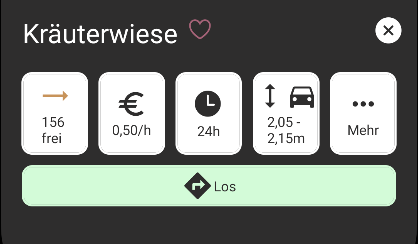
\includegraphics[width=0.45\linewidth]{parkingAreaDescriptionLetsGo_component.png}
		\caption[Die Komponente ,ParkingAreaDescription', welche bei Klick auf einen Marker aufgerufen wird.]
		{Die Komponente ,ParkingAreaDescription', welche bei Klick auf einen Marker aufgerufen wird. Hier befindet sich der Nutzer im Geofence des Parkplatzes ,Kräuterwiese' und kann über den länglichen unteren Button eine Navigation dahin starten. (Quelle: Screenshot der erstellten Anwendung.)}
		\label{fig:parkingAreaDescriptionLetsGoButton}
	\end{figure}
	\item \textbf{handleShowParkingAreaDescription(parkingAreaDescription: boolean): void} \\ Diese Funktion vom Typ ,void' mit der dazugehörigen boolschen Variable lässt diese Komponente schließen. Wird dieser Wert auf ,false' gesetzt, so ist diese Funktion dafür zuständig, dies der App mitzuteilen, welche wiederum für die Anzeige dieser Komponente zuständig ist. Es wird geprüft, ob ,parkingAreaDescription' ,true' oder ,false' anzeigt. Bei ,true' öffnet sich diese Komponente, bei ,false' wird sie geschlossen. Dies geschieht beispielsweise, wenn der kleine weiße Kreis in der rechten Ecke in \autoref{fig:parkingAreaDescriptionLetsGoButton} betätigt wird.
	\item \textbf{handleParkingAreaDetails(parkingAreaDetails: boolean): void} \\ Der boolsche Parameter der Funktion zeigt an, ob auf den ,Mehr'-Button gedrückt wird. Ist der Button gedrückt worden, so wird die Komponente ,ParkingAreaDetails' geöffnet.
	\item \textbf{handleParkingAreaData(parkingAreaData: IParkingArea): void} \\ Diese Funktion beinhaltet ein Objekt des Typs ,IParkingArea', was das Interface für einen Eintrag einer Parkmöglichkeit ist und weiter unten beschrieben wird. Die Daten zur angeklickten Parkmöglichkeit gelangen so zur ,App'.
	\newpage
	\item \textbf{handleParkingAreaDetailsData(parkingAreaDetails: IParkingAreaDetails): void} \\ Diese Property macht genau das gleiche, wie die vorherige: Es werden Daten zur ,App' getragen. In dem Fall handelt es sich um die Daten, wie voll die Parkmöglichkeit zum aktuellen Zeitpunkt ist.
	\item \textbf{handleDataBaseError(databaseError: boolean): void} \\ Diese Funktion beinhaltet einen boolschen Parameter, welcher der ,App' mitteilt, ob es zu einem Fehler in der Datenbank gekommen ist.
	\item \textbf{handleVolume(volume: boolean): void} \\ Werden die Navigation mit dem ,Los'-Button oder die Details mit dem ,Mehr'-Button geöffnet, so wird der ,App' mitgeteilt, dass der Ton der Sprachausgabe beendet werden soll. Würde dies weggelassen werden, so würde die Sprachausgabe fortgesetzt werden, wenn der Nutzer möglicherweise schon gar nicht mehr in der Anwendung, sondern schon bei der Navigation ist.
\end{description}

In der ,ParkingAreaDescription'-Komponente werden die Daten der angeklickten Parkmöglichkeit aus beiden Datenbanken abgerufen und dann in Kacheln dargestellt. Um den Code übersichtlicher zu gestalten, sind die Kacheln eine weitere Komponente: ,ParkingAreaDescriptionItemContainer', welche nachfolgend näher beschrieben wird. Zudem kann hier das Parkhaus favorisiert werden, was direkt in die Datenbank eingetragen wird. Kommt es zu einem Datenbankfehler, so wird dies dem Nutzer über ein Alert mitgeteilt. Damit die Abfrage der Datenbank klappt und die Daten vor dem Rendern in den einzelnen Komponenten der ,ParkingAreaDescription'-Komponente stehen, muss die Abfrage asynchron ablaufen. Das heißt, dass gewartet werden muss, bis die Daten da sind, bevor sie angezeigt werden.

\subsubsection{Komponente ,ParkingAreaDescriptionItemContainer'}
\label{parkingAreaDescriptionItemContainer}
Diese Komponente ist die Kachel der ,ParkingAreaDescription'. Auch sie hat ein Interface für die Properties. Dieses beinhaltet aber nur den Text, einen oder zwei Namen für Icons und die Farbe des jeweiligen Icons. Ansonsten besitzt diese Komponente keinerlei Funktionalität. Sie ist nur für das Anzeigen zuständig und, dass in der ,ParkingAreaDescription'-Komponente weniger redundanter Code ist.

\subsection{Komponente ,ParkingAreaList'}
\label{parkingAreaList}
In \autoref{fig:ParkingAreaList} ist diese Komponente zu sehen. Hier sind die Parkmöglichkeiten mit Favoriten zuerst als anklickbare Kacheln alphabetisch aufgelistet. 
\begin{figure}[h!]
	\centering
	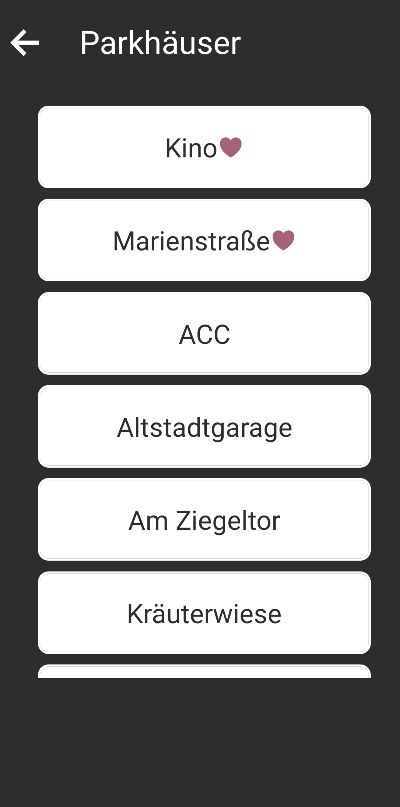
\includegraphics[width=0.33\linewidth]{parkingAreaList_component.png}
	\caption[Die Komponente ,ParkingAreaList', zu welcher über einen Klick auf das Icon oben rechts in der App navigiert wird. Die Liste ist mit Favoriten zuerst alphabetisch geordnet.]
	{Die Komponente ,ParkingAreaList', zu welcher über einen Klick auf das Icon oben rechts in der App navigiert wird. Die Liste ist mit Favoriten zuerst, alphabetisch geordnet. (Quelle: Screenshot der erstellten Anwendung.)}
	\label{fig:ParkingAreaList}
\end{figure}
\newpage
Die ,ParkingAreaList'-Komponente besitzt auch ein Interface für ihre Properties. So können die Typen dieser sichergestellt werden. Das Interface sieht folgendermaßen aus:
\begin{description}
	\item \textbf{dbConnectionService: DbConnectionService} \\ Diese Property vom Typ DbConnectionService ist wichtig für die Abfrage der Daten aus der Datenbank.
	\item \textbf{handleShowParkingAreaList(showParkingAreaList: boolean): void} \\ Diese Funktion ist dafür zuständig, die ,ParkingAreaList'-Komponente zu schließen, wenn auf den Zurück-Pfeil gedrückt wird. In \autoref{fig:ParkingAreaList} ist die Liste mit dem Zurück-Pfeil zu sehen.
	\item \textbf{handleParkingAreaDescription(parkingAreaDescription: boolean): void} \\ Die ,ParkingAreaDescription'-Komponente wird bei Drücken auf den Zurück-Pfeil geschlossen, damit die Beschreibung nicht ohne Daten geöffnet ist.
	\item \textbf{handleParkingAreaDetails(parkingAreaDetails: boolean): void} \\ Diese Funktion erfüllt denselben Zweck wie ,handleParkingAreaDetails' in \autoref{handleFunctions}.
	\newpage
	\item \textbf{handleParkingAreaData(parkingAreaData: IParkingArea): void} \\ Auch hier tut die Funktion das Gleiche, wie ,handleParkingAreaData' in \autoref{handleFunctions}.
	\item \textbf{handleParkingAreaDetailsData(parkingAreaDetails: IParkingAreaDetails): void} \\ In \autoref{handleFunctions} unter ,handleParkingAreaDetailsData' ist beschrieben, was auch diese Funktion macht.
	\item \textbf{handleDataBaseError(databaseError: boolean): void} \\ Die Beschreibung dieser Property befindet sich auch in \autoref{handleFunctions} unter ,handleDataBaseError'.
\end{description} 

Die Überschrift dieser Komponente geht aus der Komponente ,ParkingAreaListHeadig' hervor, welche in \autoref{parkingAreaListHeading} zu finden ist. Ist bei der Datenbank-Abfrage in dieser Komponente kein Fehler aufgetreten, so werden die Namen der Parkmöglichkeiten als Flatlist dargestellt. Die Kacheln, in welchen sich die Namen der Parkmöglichkeiten befinden, gehen aus der Komponente ,ParkingAreaListItem' hervor. Wird auf eine dieser Kacheln geklickt, so kommt es zu einer weiteren Abfrage der Datenbank, wobei ,handleParkingAreaData' und ,handleParkingAreaDetailsData' der eben beschriebenen Properties mit den Daten gefüllt werden. Die Property ,handleParkingAreaDetails' wird dann auf ,true' gesetzt, um die Komponente in \autoref{parkingAreaDetails} zu öffnen. Je nachdem, ob ein Fehler bei der Datenbankabfrage auftritt, wird der Parameter in ,handleDataBaseError' auf ,true' oder ,false' gesetzt.

\subsubsection{Komponente ,ParkingAreaListItem'}
\label{parkingAreaListItem}
Diese Komponente besitzt, wie alle anderen auch ein Interface. Da es sich um anklickbare Kacheln handelt, muss dieser Komponente die Funktion mitgeteilt werden, welche beim Klick ausgeführt werden soll. Für die Ausführung der Funktion braucht es zudem noch die ID der Parkmöglichkeit. Um den Namen und, falls die Parkmöglichkeit favorisiert ist, ein Herz anzuzeigen, müssen auch noch der anzuzeigende Name als String und ein numerischer Wert für die Favorisierung mitgegeben werden. 0 heißt, dass die Parkmöglichkeit nicht unter die Favoriten fällt. 1 bedeutet, dass diese favorisiert ist.

\subsection{Komponente ,ParkingAreaDetails'}
\label{parkingAreaDetails}
Wie bereits beschrieben, öffnet sich diese Komponente beim Klick auf ,mehr' in \autoref{fig:parkingAreaDescription} oder bei Auswahl einer Parkmöglichkeit in \autoref{fig:ParkingAreaList}. Diese Komponente dient lediglich zum Anzeigen von Daten. Dennoch kann auch hier eine Parkmöglichkeit zu den Favoriten hinzugefügt oder entfernt werden. Zu sehen ist diese Ansicht in \autoref{fig:parkingAreaDetails}.

\begin{figure}[h!]
	\centering
	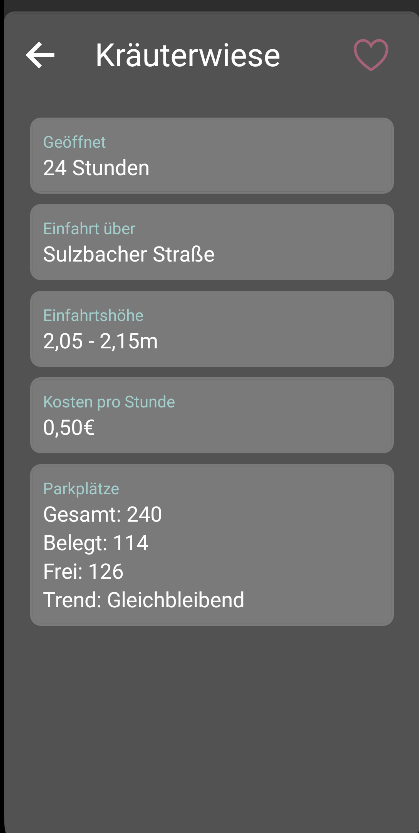
\includegraphics[width=0.33\linewidth]{parkingAreaDetails_component.png}
	\caption[Die Details zu einer Parkmöglichkeit. Hier werden alle vorhandenen Daten zur Parkmöglichkeit angezeigt. Sollte diese geschlossen sein oder aus anderen Gründen nicht befahrbar sein, wird dies dem Nutzer mit einem Text in einer roten Kachel mitgeteilt. Der Nutzer kann auch hier Parkmöglichkeiten favorisieren oder von den Favoriten entfernen.]
	{Die Details zu einer Parkmöglichkeit. Hier werden alle vorhandenen Daten zur Parkmöglichkeit angezeigt. Sollte diese geschlossen sein oder aus anderen Gründen nicht befahrbar sein, wird dies dem Nutzer mit einem Text in einer roten Kachel mitgeteilt. Der Nutzer kann auch hier Parkmöglichkeiten favorisieren oder von den Favoriten entfernen. (Quelle: Screenshot der erstellten Anwendung.)}
	\label{fig:parkingAreaDetails}
\end{figure}
\newpage
Die Properties, welche durch das Interface ihren Typ erhalten, sind folgende: 
\begin{description}
	\item \textbf{dbConnectionService: DbConnectionService} \\ Diese Propertie ist dafür zuständig, dass beim Drücken auf das Herz in der oberen rechten Ecke eine Parkmöglichkeit in der Datenbank als Favorit oder kein Favorit eingetragen werden kann.
	\item \textbf{handleShowParkingAreaDetails(parkingAreaDetails: boolean): void} \\ Diese Funktion wird benötigt, wenn der Pfeil in der oberen linken Ecke gedrückt wird. Tut der Nutzer das, so wird ,parkingAreaDetails' auf ,false' gesetzt und die Ansicht aus \autoref{fig:parkingAreaDetails} wird geschlossen.
	\item \textbf{parkingAreaData: IParkingArea} \\ Das Objekt, welches Parkhausdaten, wie die Einfahrtshöhe oder den Preis, beinhaltet.
	\item \textbf{parkingAreaDetailsData: IParkingAreaDetails} \\ Das Objekt, welches die Daten der API beinhaltet, welche unter ,Parkplätze' in \autoref{fig:parkingAreaDetails} dargestellt sind.
	\newpage
	\item \textbf{databaseError: boolean} \\ Ist diese Property ,true', so bekommt der Nutzer eine rot gefärbte Kachel mit einem Text angezeigt, der ihn darauf hinweist, dass die Daten nicht angezeigt werden können. In diesem Fall ist die Aktion zu wiederholen.
\end{description}

Da hier die Kacheln ebenfalls aus jeweils den gleichen ,View'-Komponenten und demselben Design bestehen, wird hier wieder eine Komponente ,ParkingAreaDetailsItem' erstellt, welche sich darum kümmert, die Elemente einheitlich anzuzeigen. Die Überschrift kommt ebenfalls durch die Komponente ,ParkingAreaListHeading' in \autoref{parkingAreaListHeading} zustande, wie die Überschrift in \autoref{parkingAreaList}.

\subsubsection{Komponente ,ParkingAreaDetailsItem'}
Diese Komponente ist ebenfalls nur zum Anzeigen von Dateien. Ihre Properties sind der Text, der in der Kachel jeweils oben kleiner angezeigt wird und jener Text, welcher etwas größer darin steht und abhängig von der angeklickten Parkmöglichkeit ist. Außerdem wird eine boolsche Variable hineingegeben, die dieser Komponente mitteilt, ob es sich um die Anzeige eines Fehlers handelt. Ist das der Fall, werden die Kacheln rot gefärbt.

\subsection{Komponente ,ParkingAreaListHeading'}
\label{parkingAreaListHeading}
Diese Komponente beinhaltet das Design der Überschrift, wie in \autoref{fig:ParkingAreaList} oder \autoref{fig:parkingAreaDetails} zu sehen. Als Property werden hier lediglich die Funktion, die beim Klick auf den Zurück-Pfeil erfolgen soll und der Text, welcher dargestellt werden soll, hineingegeben.

\section{Datenbankverbindung ,DbConnectionService'}
Zur Speicherung der Daten der Parkmöglichkeiten wird SQLite verwendet. Sämtliche Funktionen, die Datenbankzugriff benötigen, sind in der Klasse ,DbConnectionService' niedergeschrieben. Mit Hilfe eines Beispiels in dieser Expo-Bibliothek konnte eine Datenbank erstellt werden, wie in \autoref{lst:openDatabase} zu sehen. Diese Funktion wird im Konstruktor der Klasse aufgerufen. eine Instanz der Klasse wird in der ,App' erstellt und an alle Komponenten, die Datenbankzugriff benötigen, weitergegeben.

\begin{lstlisting}[caption={Das Erstellen einer Datenbank mit Hilfe eines Beispiels der genutzten Expo-Bibliothek SQLite. (Quelle: \cite{sqlite})},captionpos=b, language=Java, label=lst:openDatabase]
private openDatabase = () => {
	if (Platform.OS === "web") {
		return {
			transaction: () => {
				return {
					executeSql: () => {},
				};
			},
		};
	}
	const db = SQLite.openDatabase("db.db");
	return db;
};
\end{lstlisting}

Diese Klasse besitzt folgende Funktionen:
\begin{description}
	\item \textbf{public createTables()} \\ Mit dieser Funktion werden die Tabellen ,parkingarea' und ,parkingareadetails' mit einem SQL-Befehl erstellt, falls diese nicht existieren. Ist die Tabelle ,parkingarea' leer, so wird diese mit den Daten des Objekt-Arrays aus \autoref{AllParkingAreas} gefüllt.
	\item \textbf{public getData()} \\ Hier werden die Daten der API mittels ,fetch()' geholt und mit einem XML-Parser in ein Objekt umgewandelt \cite{xmlParser}. Um die Umlaute im Namen und dem Status für einen Nutzer leserlich zu machen, wird das Encoding danach noch geändert \cite{htmlEntities}. Anschließend werden die Daten in die Tabelle ,parkingAreaDetails' mit Hilfe der folgenden Funktion eingefügt.
	\item \textbf{private insertIntoDetailsTable(name: string, dateOfData: string, numberOfLots: number, numberOfTakenLots: number, numberOfFreeLots: number, trend: number, status: string, closed: number, ctr: number)} \\ Mit dieser Funktion werden die Daten in die Tabelle ,parkingareadetails' eingefügt. Danach wird der jeweils älteste Datensatz gelöscht, sodass pro Parkhaus nur drei Datensätze existieren. Das ist wichtig, da dann in jedem Fall Daten angezeigt werden können, auch, wenn diese schon älter sind. Der Nutzer sieht also immer direkt Daten und nicht nur leere Elemente.
	\item \textbf{public async getDataFromParkingAreaTable(parkingAreaId: number)} \\ Mit Hilfe der ID wird in der Tabelle ,parkingarea' nach der richtigen Parkmöglichkeit gesucht. Die Daten werden in einem Objekt des Typs ,IParkingArea' gespeichert. Da diese Funktion asynchron ist, gibt sie ein Promis zurück. Dies ist notwendig, da sonst die Benutzeroberfläche gerendert sind, bevor die Datenbankabfrage getätigt werden kann. So wird zunächst die Abfrage getätigt und danach die Benutzeroberfläche gerendert.
	\item \textbf{public async getDataFromParkingAreaDetailsTable(parkingAreaId: number)} \\ Diese Funktion tut dasselbe wie ,public async getDataFromParkingAreaTable (parkingAreaId: number)'. Nur werden hier die Daten aus der ,parkingareadetails'-Tabelle genommen und in einem Objekt des Typs ,IParkingAreaDetails' gespeichert.
	\item \textbf{public async getParkingAreas()} \\ Aus oben genannten Gründen ist auch diese Funktion wieder asynchron. Diese Abfrage liefert alle Parkmöglichkeiten der ,parkingarea'-Tabelle geordnet nach Favoriten und Namen. Dieses Ergebnis hat den Typ ,SQLResultSetRowList', welcher aus der SQLite Bibliothek kommt, und kann mit dem Anhang ,.\_array' in ein Array umgewandelt werden.
	\item \textbf{public setFavoriteParkingArea(favorite: number, name: string)} \\ Diese Funktion ist für das Updaten der Parkmöglichkeit zuständig. Mit einem SQL-Befehl wird die Parkmöglichkeit mit dem mitgegebenen Namen ,name' aktualisiert und der Wert, ob die Parkmöglichkeit favorisiert wird oder nicht, wird auf ,favorite' gesetzt. Hierbei bedeutet 0 kein Favorit und 1, dass die Örtlichkeit favorisiert ist.
\end{description}

Bei jeglichen Datenbankfehlern wird ein Alert ausgegeben, um dem Nutzer mitzuteilen, dass etwas schief gelaufen ist. In so einem Fall empfiehlt es sich, die Aktion zu wiederholen oder die App neu zu starten \cite{sqlite}.

\section{Eventhook ,useGeofenceEvent'}
\label{geofenceEvent}
Dies ist der selbstdefinierte Hook, der die Daten vom Taskmanager in die App bring, in der sie weiter verteilt werden können. In der ,ParkingMap'-Komponente wird das Geofencing mit einem Task gestartet. Im Hook wird der Task mit demselben Task-Namen definiert. Zudem gibt es ein Array mit Funktionen, die im Task abgearbeitet werden sollen. Vor der Definition des Hooks findet sich also der Code aus \autoref{lst:taskmanager}.

\begin{lstlisting}[caption={Dieser Code befindet sich vor der Definition des Eventhooks. Hier wird ein Array angelegt, welches Funktionen beinhaltet. Diese werden dann ab Zeile 11 im definierten Task abgearbeitet. (Quelle: Eigene Implementierung)},captionpos=b, language=Java, label=lst:taskmanager]
	let geofenceHandles: TaskManager.TaskManagerTaskExecutor[] = [];
	
	TaskManager.defineTask(configStrings.geofenceTask, (data) => {
		for (const handle of geofenceHandles) {
			handle(data);
		}
	});
\end{lstlisting}

Im Eventhook werden dann zunächst Variablen definiert: Ein ,useState' vom Typ ,IEventData' und ein Objekt vom Typ ,IEventData'. Dies ist notwendig, da bei Verwendung des Emulators bei höheren Abspielgeschwindigkeiten des Abfahrens der Route ein Geofence fälschlicherweise mehrmals betreten wird und so das Event mehrmals ausgelöst wird. Die Daten des ,useState' aktualisieren sich jedoch nicht schnell genug, um zu überprüfen, ob das Geofence zum zweiten Mal hintereinander betreten und nicht verlassen wird. Aus diesem Grund wird das Objekt benötigt. Jedoch kann der ,useState' auch nicht weggelassen werden, da in der ,App' keine Daten ankommen, wenn nur das Objekt verwendet wird. 

Als nächstes wird dann ein ,useEffect' erstellt, in dem eine Funktion ,handleIsInGeofence' definiert wird. Diese ist in \autoref{lst:handleIsInGeofence} in \autoref{appendix:geofencing} zu erkennen. Im Fehlerfall wird ein Toast ausgegeben, der dem Nutzer mitteilt, dass das Geofencing gerade nicht möglich ist. Von Zeile 10 bis 17 wird überprüft, ob das Geofence mehrmals hintereinander betreten wird. Ist das der Fall, so kommt es zu einem ,return' in Zeile 15. Ab Zeile 19 steht, was beim Betreten von Geofences passiert: Das Objekt und der ,useState' werden aktualisiert und der Nutzer bekommt mit einem Toast mitgeteilt, wo er sich befindet. Verlässt der Nutzer das Geofence, so tritt der Code ab Zeile 30 in Kraft. Hier werden nur die Daten des Objekts und des ,useStates' aktualisiert. Anschließend wird die Funktion ,handleIsInGeofence' zu dem oben angelegten Array aus Funktionen hinzugefügt, um vom Taskmanager abgearbeitet zu werden. Danach wird die Funktion aus dem Array entfernt.

Der Eventhook gibt den ,useState' zurück und die benötigten Daten landen in der ,App', wo sie in ein Array aus Objekten aller Parkmöglichkeiten übertragen werden. Bei jeder Parkmöglichkeit bei der ,ParkingAreaDescription'-Komponente wird so der ,Los'-Button aus \autoref{fig:parkingAreaDescriptionLetsGoButton} angezeigt, wenn sich der Nutzer im Geofence befindet.

\section{Models}
Damit die Datentypen von Objekten stimmen, werden Models in Form von Interfaces erstellt. Das hilft, um mehrfach benutzten Objekten immer denselben Datentyp mitzugeben. Der Entwickler wird so zudem schneller auf Unstimmigkeiten bezüglich des Datentyps aufmerksam gemacht.

\subsection{Interface ,IParkingArea'}
\label{iParkingArea}
Mit ,IParkingArea' erstellte Objekte beinhalten alle Daten der Parkmöglichkeiten, die sich gar nicht oder seltener ändern. Diese sind in der nachfolgenden \autoref{tab:iParkingArea} dargestellt. Die Schlüssel sind hierbei dieselben, wie die Spalten in der Datenbanktabelle ,parkingarea'.

\begin{center}
	\begin{table*}[h!]
		\centering
		\begin{NiceTabular}{|r||l|}
			\CodeBefore
			\rowcolor{lightgray}{1}
			\Body\Hline
			\textbf{Schlüssel} 		 & \textbf{Datentyp}	\\\Hline\Hline
			id				 	& number					\\\Hline
			name			 	& string					\\\Hline
			address	 			& string 					\\\Hline
			openingHours		& number					\\\Hline
			pricePerHour		& string					\\\Hline
			doorHeight			& string					\\\Hline
			favorite			& 0 | 1						\\\Hline
			lat			 		& number					\\\Hline
			long 		 		& number					\\\Hline
		\end{NiceTabular}
		\vspace*{1em}
		\caption{Die Schlüssel und ihre Datentypen des Interfaces ,IParkingArea'.}
		\label{tab:iParkingArea}
	\end{table*}
\end{center}  

\subsection{Interface ,IParkingAreaDetails'}
Auch hier orientieren sich die Datentypen und die Schlüssel wieder an einer Datenbanktabelle. In diesem Fall ist das ,parkingareadetails', wie in \autoref{tab:iParkingAreaDetails} erkennbar ist.

\begin{center}
	\begin{table*}[h!]
		\centering
		\begin{NiceTabular}{|r||l|}
			\CodeBefore
			\rowcolor{lightgray}{1}
			\Body\Hline
			\textbf{Schlüssel} 		 & \textbf{Datentyp}								\\\Hline\Hline
			id				 	& number												\\\Hline
			parkingAreaId	 	& number												\\\Hline
			numberOfLots		& number 												\\\Hline
			numberOfTakenLots	& number												\\\Hline
			numberOfFreeLots	& number												\\\Hline
			trend				& 0 | 1 | -1											\\\Hline
			status				& ''OK'' | ''Ersatzwerte'' | ''Manuell'' | ''Störung''	\\\Hline
			closed		 		& 0 | 1													\\\Hline
			dateOfData	 		& string												\\\Hline
		\end{NiceTabular}
		\vspace*{1em}
		\caption{Die Schlüssel und Datentypen des Interfaces ,IParkingAreaDetails'.}
		\label{tab:iParkingAreaDetails}
	\end{table*}
\end{center}  

\subsection{Interface ,IEventData'}
Da dieses Interface, wie oben beschrieben, auch häufiger benutzt wird, ist es in eine extra Datei gewandert. Benötigt wird es für den Umgang mit den Geofences. Dieses Interface besitzt zwei Schlüssel mit Datentypen, wie in \autoref{tab:iEventData} zu sehen.

\begin{center}
	\begin{table*}[h!]
		\centering
		\begin{NiceTabular}{|r||l|}
			\CodeBefore
			\rowcolor{lightgray}{1}
			\Body\Hline
			\textbf{Schlüssel} 		 & \textbf{Datentyp}	\\\Hline\Hline
			parkingAreaName		& string					\\\Hline
			enteredParkingArea	& boolean					\\\Hline
		\end{NiceTabular}
		\vspace*{1em}
		\caption{Die Schlüssel und Datentypen des Interfaces ,IParkingAreaDetails'.}
		\label{tab:iEventData}
	\end{table*}
\end{center}

\section{Parkhausdaten ,AllParkingAreas'}
\label{AllParkingAreas}
Damit die Marker der ,ParkingMap' gesetzt und die Daten in die Datenbanktabelle ,parkingarea' eingefügt werden können, werden die Daten der Parkmöglichkeiten benötigt. Diese befinden sich in einer TypeScript-Datei, da dies hilft, die Datentypen zu bewahren. Die Darstellung der Daten ist wie bei einer JSON-Datei. Dennoch gibt es so die Möglichkeiten, Datentypen für die Werte der einzelnen Schlüssel festzulegen. Als Interface für die Werte wird ,IParkingArea' aus \autoref{iParkingArea} verwendet. In \autoref{lst:allParkingAreas} ist diese Datei verkürzt dargestellt. 

\begin{lstlisting}[caption={Die verkürzte Darstellung der Datei, welche die Daten der Parkmöglichkeiten beinhaltet. Wäre Typensicherheit egal, könnten die Daten auch in eine JSON-Datei geschrieben werden. (Quelle: Eigene Implementierung)},captionpos=b, language=Java, label=lst:allParkingAreas]
	import { IParkingArea } from "./models/IParkingArea";
	
	export const allParkingAreas: IParkingArea[] = [
	{
		id: 4,
		name: "Am Ziegeltor",
		address: "Pfalzgrafenring",
		openingHours: 24,
		pricePerHour: "0,50",
		doorHeight: "2,10",
		favorite: 0,
		lat: 49.44854933741437,
		long: 11.856581325108372,
	},
	{
		id: 8,
		name: "Altstadtgarage",
		address: "Kaiser-Ludwig-Ring",
		openingHours: 24,
		pricePerHour: "1,00",
		doorHeight: "2,00",
		favorite: 0,
		lat: 49.447409726965354,
		long: 11.861757130222472,
	},
];	
\end{lstlisting}

\section{Zentrale Verwaltung der Farben und Strings}
Damit die Farben und Strings bei Änderungen nicht an jeder Stelle im Quellcode geändert werden müssen, werden diese zentral in zwei Dateien verwaltet. In der ,colors'-Datei finden sich die Farben als gleichnamiges Objekt. Hierzu gibt es Schlüssel-Wert-Paare mit Bezeichnungen der Farben und den Farbwerten. 

Bei den Strings in der ,strings'-Datei gilt dasselbe Prinzip. Hier gibt es aber mehrere Objekte, da die Texte gruppiert sind. Die Gruppierungen sind Folgende:

\begin{description}
	\item \textbf{sqlQuerys} \\ Dieses Objekt enthält alle verwendeten SQL-Befehle. Sollte sich etwas daran ändern, kann das hier geschehen und es muss nicht im Code nach dem Befehl gesucht werden.
	\item \textbf{configStrings} \\ Diese Kategorie enthält die API mit den Daten der Parkplätze der Parkmöglichkeiten und den Namen des Tasks, der für das Geofencing benutzt wird.
	\item \textbf{errorMessages} \\ In diesem Objekt finden sich alle Fehler- und Warnmeldungen wieder.
	\item \textbf{outputText} \\ Hier befinden sich alle weiteren Texte, die dem Nutzer im Laufe der Benutzung der Anwendung angezeigt werden.
\end{description}